\documentclass[class=article, crop=false]{standalone}
\usepackage[subpreambles=true]{standalone}
\usepackage{import}
\usepackage{blindtext}
% images
\usepackage{graphicx}
\begin{document}


\section{La récupération des données}

Parler de la récupération des données depuis les deux APIs discutés (cf.\,fig.~\ref{fig:workflow}) ainsi que le fichier YAML de configuration.

\begin{figure}
\centering
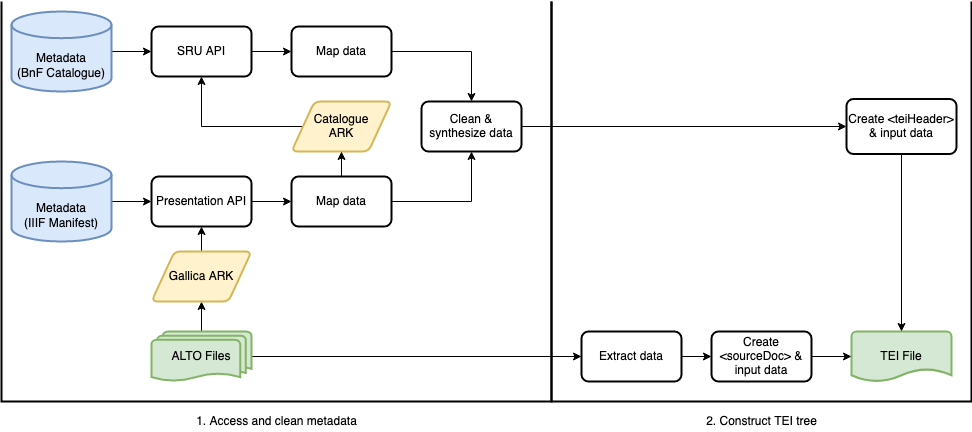
\includegraphics[width=\textwidth]{../../../images/full_tree.png}
\label{fig:workflow}
\caption{Workflow}
\end{figure}

\subsection{Du manifest IIIF à un dictionnaire Python}

Montrer le mapping des données du manifest au dictionnaire Python.

\subsection{De l'Unimarc à un dictionnaire Python}

Montrer le mapping des données du catalogue au dictionnaire Python.

\section{L'analyse des données}

Parler de la stratégie d'atténuation des risques en sélectionnant les données fiables. Les métadonnées du catalogue général de la BnF sont utilisées uniquement si le même exemplaire physique du document numérisé sur Gallica a bien été trouvé. Sinon, on risque de mettre les données d'un autre exemplaire de l'oeuvre que celui qui a été transcrit et donc introduire des fausses données, tel que le cote ou même l'éditeur et la date de publication de l'exemplaire.

\section{Le modèle du \texttt{<teiHeader>}}

Montrer le mapping des données au \texttt{<teiHeader>}.

\end{document}
\documentclass[../main.tex]{subfiles}